\documentclass[preprint,12pt]{elsarticle}
% major revision and answer question (3 reviewers)
%Sunday, January 24⋅22:30 – 22:55
%Daily, until Jan 29, 2021

% mark in blue or red
\usepackage{xcolor}

\newenvironment{MyColorPar}[1]{%
    \leavevmode\color{#1}\ignorespaces%
}{%
}%

%%% for abbreviations, or acronyms
\usepackage[automake, acronym, nopostdot]{glossaries} 
%\usepackage{glossary-inline}
%\newenvironment{abbreviation}
%\makeglossaries %https://tex.stackexchange.com/questions/110095/list-of-acronyms-is-not-displayed
\newacronym{fdr}{FDR}{false discovery rate}
\newacronym{hpa}{HPA}{the Human Protein Atlas}
\newacronym{hnscc}{HNSCC}{head and neck squamous cell carcinoma}
\newacronym{tcga}{TCGA}{the Cancer Genome Atlas}
\newacronym{tcpa}{TCPA}{the Cancer Proteome Atlas}
\newacronym{rna}{RNA}{ribonucleic acid}
\newacronym{rnaseq}{RNA-Seq}{RNA sequencing}
\newacronym{lncrna}{lncRNA}{long non-coding RNA}
%\newacronym{km}{KM}{Kaplan-Meier}
\newacronym{rppa}{RPPAs}{reverse-phase protein arrays}
\newacronym{rpma}{RPMA}{reverse-phase protein lysate microarray}

\newacronym{mmp}{MMP}{matrix metalloproteinase}
 %DKK1, CAMK2N1, STC2, PGK1, SURF4, USP10, NDFIP1, FOXA2, STIP1, and DKC1
 %ZNF557, ZNF266, IL19, MYO1H, FCGBP, LOC148709, EVPLL, PNMA5, KIAA1683, and NPB

\newacronym{DKK1}{DKK1}{dickkopf WNT signaling pathway inhibitor 1} 
\newacronym{CAMK2N1}{CAMK2N1}{calcium/calmodulin dependent protein kinase II inhibitor 1} 
\newacronym{STC2}{STC2}{stanniocalcin 2} 
\newacronym{PGK1}{PGK1}{phosphoglycerate kinase 1} 
\newacronym{SURF4}{SURF4}{surfeit 4} 
\newacronym{USP10}{USP10}{ubiquitin specific peptidase 10} 
\newacronym{NEDD4}{NEDD4}{neural precursor cell expressed, developmentally down-regulated 4}
\newacronym{NDFIP1}{NDFIP1}{NEDD4 family interacting protein 1} 
\newacronym{FOXA2}{FOXA2}{forkhead box A2} 
\newacronym{STIP1}{STIP1}{stress-induced-phosphoprotein 1} 
\newacronym{DKC1}{DKC1}{dyskeratosis congenita 1, dyskerin} 

\newacronym{ZNF557}{ZNF557}{zinc finger protein 557} 
\newacronym{ZNF266}{ZNF266}{zinc finger protein 266} 
\newacronym{IL19}{IL19}{interleukin 19} 
\newacronym{MYO1H}{MYO1H}{myosin 1H} 
\newacronym{FCGBP}{FCGBP}{Fc fragment of IgG binding protein} 
\newacronym{LOC148709}{LOC148709}{LncRNA LOC148709} 
\newacronym{EVPLL}{EVPLL}{envoplakin-like protein} 
\newacronym{PNMA5}{PNMA5}{paraneoplastic antigen like 5} 
%\newacronym{KIAA1683}{KIAA1683}{IQCN, IQ Motif Containing N} 
\newacronym{IQCN}{IQCN}{IQ motif containing N} % previous name KIAA1683
% "IQ" refers to the first two amino acids of the motif: isoleucine (commonly) and glutamine (invariably)
\newacronym{NPB}{NPB}{neuropeptide B} 

 \newacronym{rt}{RT}{radiation therapy}
 \newacronym{nccn}{NCCN}{National Comprehensive Cancer Network}
 \newacronym{hif}{HIF}{hypoxia-inducible factor}
 \newacronym{egfr}{EGFR}{epidermal growth factor receptor}
 \newacronym{ras}{RAS}{rat sarcoma}
 \newacronym{hras}{HRAS}{Harvey rat sarcoma viral oncoprotein}
 \newacronym{erk}{ERK}{extracellular signal-regulated kinases}
 \newacronym{us}{US}{United States}
 \newacronym{fda}{FDA}{Food and Drug Administration}
 \newacronym{tpf}{Tax-PF}{docetaxel, cisplatin, and 5-fluorouracil}
 \newacronym{tki}{TKI}{tyrosine kinase inhibitor}
 \newacronym{her}{HER}{human epidermal growth factor receptor}
 \newacronym{ici}{ICI}{immune-checkpoint inhibitor}
 \newacronym{ctla4}{CTLA-4}{cytotoxic T lymphocyte antigen 4}
 \newacronym{pd1}{PD-1}{programmed death 1}
 \newacronym{pdl1}{PD-L1}{programmed death ligand 1}
 \newacronym{tim3}{TIM-3}{T-cell immunoglobulin mucin protein 3}
 \newacronym{lag3}{LAG-3}{lymphocyte activation gene 3}
 \newacronym{ifng}{IFN-$\gamma$}{interferon gamma}
 \newacronym{tigit}{TIGIT}{T cell immunoglobin and immunoreceptor tyrosine-based inhibitory motif}
 \newacronym{gitr}{GITR}{glucocorticoid-induced tumor necrosis factor receptor}
 \newacronym{vista}{VISTA}{V-domain Ig suppressor of T-cell activation}
 \newacronym{tmsb4x}{TMSB4X}{thymosin beta-4 X-linked}
 \newacronym{emt}{EMT}{epithelial-mesenchymal-transition}
 \newacronym{gdc}{GDC}{Genomic Data Commons}
 \newacronym{nci}{NCI}{the National Cancer Institute}
 \newacronym{gdac}{GDAC}{Genome Data Analysis Center}
 \newacronym{rest}{REST}{Representational State Transfer} 
 \newacronym{api}{API}{Application Programmable Interface}
\newacronym{grch38}{GRCh38}{Genome Reference Consortium Homo sapiens genome assembly 38}
\newacronym{fpkm}{FPKM}{Fragments per kilobase per million reads mapped}
\newacronym{rsem}{RSEM}{RNA-Seq by Expectation-Maximization}
\newacronym{slca}{SLC35E2A}{solute carrier family 35 member E2A}
\newacronym{slcb}{SLC35E2B}{solute carrier family 35 member E2B}
\newacronym{cde}{CDE}{Common Data Element}
\newacronym{id}{ID}{identification}
\newacronym{ajcc}{AJCC}{the American Joint Committee on Cancer}
\newacronym{uicc}{UICC}{he Union for International Cancer Control}
\newacronym{tnm}{TNM}{the tumor size (T), cervical lymph node metastases (N), and distal metastasis status (M)}
\newacronym{ci95}{95\% CI}{95\% confidence interval}
\newacronym{os}{OS}{overall survival}
\newacronym{hr}{HR}{hazard ratio}
\newacronym{hpv}{HPV}{human papillomavirus}
\newacronym{ene}{ENE}{extra-nodal extension}
\newacronym{lvsi}{LVSI}{lymph-vascular space invasion}
\newacronym{pni}{PNI}{perineural invasion}
\newacronym{doi}{DOI}{depth of invasion}
\newacronym{lnd}{LND}{lymph node density}
\newacronym{wpoi5}{WPOI-5}{worst pattern of invasion score 5}
\newacronym{glut4}{GLUT4}{glucose transporters 4}
\newacronym{slc2a4}{SLC2A4}{solute carrier family 2 member A4}
\newacronym{trim24}{TRIM24}{tripartite motif-containing 24}
\newacronym{til}{TIL}{tumor-infiltrating lymphocytes}
\newacronym{tmb}{TMB}{tumor mutational burden}



%==================
\begin{document}

\section{Revision cover letter (cancers-1082127)} % 2021/01/25
%其實直接 online 填寫即可
%Please provide a cover letter to explain point-by-point the details of the revisions [changes 摘要即可 from the rebuttal]  in the manuscript
 

%Assistant Editor
%E-Mail: aubree.zhu@mdpi.com
%MDPI Branch Office, Tianjin
Assistant Editor of Cancers%\newline

Jan 29, 2021

Dear Dr. Aubree Zhu:

Enclosed, please find our revised manuscript (cancers-1082127) entitled "A Global Genome-wide Scan with Optimal Cutoff Mining for Emerging Biomarkers in Head and Neck Squamous Cell Carcinoma" by Chi et al., which we wish to be considered for publishing as a research article in Cancers. We greatly appreciate your time in serving as the editor handling this manuscript and also thank the reviewers for their critical comments and suggestions on our manuscript.

We have since performed additional analysis, experiment and revised the manuscript accordingly to address their critical comments and suggestions in a point-by-point manner, 
%

According to the editor's comments, we have the manuscript checked for English grammar and reformat Table 1 by rotating 90 degrees to portrait mode. %(Table 1 轉正)

%

We wish our revised manuscript could be satisfied and accepted for publication in Cancers. Thanks very much for the kind helps and the reviewers' critical comments.

Kind regards,

Yu-Chuan (Jack) Li, M.D., Ph.D.

Graduate Institute of Biomedical Informatics, 

College of Medical Science and Technology,

Taipei Medical University,

Taipei, Taiwan

%2) [cancers-1082127_main_redMarked] 自動化 by latex:
%"Track Changes" function in latex => by latexdiff
%Some options, taken from the documentation, include:
%UNDERLINE—added text is wavy-underlined and blue, discarded text is struck out and red;
%CTRADITIONAL—added text is blue and set in sans-serif, and a red footnote is created for each discarded piece of text;
%TRADITIONAL—like CTRADITIONAL but without the use of colour;
%CFONT—added text is blue and set in sans-serif, and discarded text is red and very small size;
%FONTSTRIKE—added text is set in sans-serif, discarded text small and struck out;
%CHANGEBAR—added text is blue, and discarded text is red. Additionally, the changed text is marked with a bar in the margin.
%https://www.overleaf.com/learn/latex/Articles/Using_Latexdiff_For_Marking_Changes_To_Tex_Documents

\pagebreak

\section{rebuttal} % Response2Referees
We greatly appreciate the reviewers for their helpful suggestions and critical comments on our manuscript. The detailed point-by-point reply to the reviewer’s comments are as follows (marked as \textcolor{blue}{blue}). 
And the revised portions in the manuscript are indicated in \textcolor{red}{red}.

%Reviewer #1(Technical Comments to the Author):
%   The ms investigates an interesting and timely topic. However, the discovery cohort involves a small sample size and throughout the analysis, the issue of correcting the obtained p-values for multiple comparisons is not addressed. Hence, the evidence for zooming into TMSB4X is not convincing.

%\section{Responses to Reviewers' comments}
% our responses to the reviewers' comments.
%***Response to reviewer's comments: [藍色字]

Comments from the reviewer \#1:

Comments and Suggestions for Authors
The authors have described the effectiveness of RNA sequencing as a tool for exploring prognostic factors; they have also performed a large-scale analysis using the TCGA cohort, which is a very attractive analysis method. I have a few minor questions.

This is an attractive analysis method and I would like to know more details.

\subsection*{1-1}
It is generally known that high expression of EGFR is a poor prognostic factor in head and neck cancers, however, why is it that RNA sequencing does not identify RNA coding for EGFR as a poor prognostic factor?

\begin{MyColorPar}{blue}
Answer

We appreciate the reviewer for the critical comments and thank for his/her agreement of our analysis using the TCGA cohort.
%[我的 candidate 中為什麼沒有 EGFR];  
In our analysis, the \acrshort{egfr} is ranked at 5707 from 20500 protein-coding genes %5708-1
by Kaplan-Meier estimate with the log-rank test P-value as 0.0495. The \acrshort{egfr} is identified as one of those poor prognostic factors as well. %However, it is far from the top 20 candidates.
(please see https://github.com/texchi2/\linebreak
pvalueTex/blob/master/HNSCC\_OS\_marginS\_6429.csv for reference, the table was ranked by FDR P-value)

% transforming growth factor- (TGF-α) 
% epidermal growth factor receptor (EGFR)
As in our manuscript mentioned, 
In a multivariate analysis, tumor site, tumor level of \acrshort{egfr}, and tumor level of TGF-$\alpha$ (\acrshort{egfr} ligand) were statistically significant predictors of disease-free survival of \acrshort{hnscc} patients\cite{Rusch1996}\cite{Grandis1998}.
Since that breakthrough discovery and validation, the \acrshort{egfr} monoclonal antibody (cetuximab)\cite{Bonner2006a} and \acrshort{egfr} \acrshort{tki} (such as gefitinib, erlotinib, osimertinib) were developed to treat advanced \acrshort{hnscc}. Although 90\% of \acrshort{hnscc} has overexpression of \acrshort{egfr}, cetuximab has only 10\% to 20\% response rate on those patients\cite{Johnson2020}. So far, cetuximab is still the only drug of choice with proven efficacy, which targeted the selected \acrshort{hnscc} patients\cite{Taberna2019}.
%citing the line number and exact change, marked in \textcolor{red}{Red from page 6 (line 16) to page 7 (line 17)}
Thus, we wish the further validations of our meaningful hypotheses of candidate to explore more useful drug of choice in the treatment of \acrshort{hnscc} patients.
% a list from literature review, 留 下少於  50 articles mentioned candidates
%HNSCC_survivalAnalysis_marginS_EGFR.Rda
%HNSCC_survivalAnalysis_marginS_EGFR.xlsx
%https://github.com/texchi2/pvalueTex/blob/master/file20500_list.txt
%analysis_export.R to generate https://github.com/texchi2/pvalueTex/blob/master/HNSCC_OS_marginS_6429.csv
\end{MyColorPar}


\subsection*{1-2}
 DNA alteration (mutation/amplification) is also an influential prognostic factor, but I would like to know if DNA alteration is considered in this analysis.
%[如果加入 DNA alteration 又會如何? 不佳; 選擇 mRNA 的原因是? interpretability and drugable: EGFR]

\begin{MyColorPar}{blue}
Answer

We appreciate the reviewer for reminding the importance of DNA alteration in survival analysis.
Those different types of omics data measured for the same patients (called multi-omics data) are currently under investigation across several disciplines such as genomics (i.e. DNA mutation/amplification, single nucleotide polymorphisms), %copy number variation), 
epigenomics, transcriptomics (i.e. RNA expression), proteomics, metabolomics and microbiomics.
The usefulness of multi-omics data for the prediction of HNSCC outcome is expected.
%such as the (censored) survival time.
Moritz Herrmann et al.(2020) observed that using multi-omics and survival data can slightly improve the performance of prediction methods for particular datasets, such as TCGA HNSCC\cite{Herrmann2020}.
%It is limited that the utility of multi-omics data for prediction purposes in the considered TCGA studies\cite{Herrmann2020}.
%18 cancer datasets from The Cancer Genome Atlas (TCGA) 
According to their study, %the multi-omics structure have a slightly better prediction performance than naive (0.562 vs.	0.557 ) with favoring clinical variables leads to better prediction results for HNSCC. %likelihood-based boosting (CoxBoost and CoxBoost favoring)
% Exemplary t-tests comparing blockForest with CoxBoost favoring and the Clinical only model showed no significant differences in performance. 
% blockForest also offers the possibility of favoring clinical covariates using the argument always.select.block of the blockfor function
%Last but not the least, multi-omics data are structured: the variables are partitioned into (non overlapping) groups. 
% ***
the survival analysis of TCGA HNSCC dataset by blockForest method (with multi-omics and clinical variables) has a similar prediction performance than that by Cox's model (with clinical variables alone). %from The Cancer Genome Atlas (TCGA) 
They also reported the performance C-index as 0.582 [CI: 0.554, 0.610] in blockForest method and 0.554 [CI: 0.519, 0.588] in Cox's model\cite{Herrmann2020}.

% 小心光茫太甚  Well-established prognostic clinical variables: prioritize
% the number of variables in the group of variables of TCGA HNSCC dataset:
% 11 clinical variables, 57964 CNV variables, 17248 mutation variables and 21520 RNA expression variables.
%*** Taking this structure into account can protect the predictive information that transcriptomics (e.x. RNA-Seq) or low-dimensional clinical variables might get lost within the huge amount of genomics (e.x. DNA mutation/amplification, copy number variation) data\cite{Boulesteix2011}\cite{Herrmann2020}.
DNA amplification will usually be one of the causes to overexpress the gene.
Moreover, transcriptomics study is helpful in drug discovery. For example, the overexpressed gene is possible to be a drug-targetable candidate\cite{Park2015}. After thoughtful validation in vitro/in vivo then pathway study, the EGFR inhibitory leads were constructed by antibody design or chemical compound screening\cite{Mahajan2016}. %比較容易研發 clinical and transcriptomics by ssurvival::survfit and urvival::coxph
% the selection of clinicalfeatures by domain knowledge and studies where HNSCC was under investigation.
The discovery of EGFR inhibitors\cite{Bonner2006a} for HNSCC therapy will encourage research community to conduct the survival analysis under abnormality in gene expression.

% *** it needs deep learning, but less interpretability (yet under development\cite{Chaudhary2018}) (DNA+RNA and clinical dataset => multi-omics cancer study)
%high dimensional multi-omics analysis by deep learning 
%It may be beneficial to include these different data types in models predicting outcomes, such as the survival time of patients. Until recently, only data from a single omics type were used to build such prediction models, with or without the inclusion of standard clinical data [2]. In recent years, however, the increasing availability of different types of omics data measured for the same patients (called multi-omics data from now on) has led to their combined use for building outcome prediction models. An important characteristic of multi-omics data is the high-dimensionality of the datasets, which frequently have more than 10 000 or even 100 000 variables. This places particular demands on the methods used to build prediction models: they must be able to handle data where the number of variables by far exceeds the number of observations. Moreover, practitioners often prefer sparse and interpretable models containing only a few variables [3]. Last but not the least, multi-omics data are structured: the variables are partitioned into (nonoverlapping) groups. This structure may be taken into account when building prediction models.
%Citation: https://academic.oup.com/bib/advance-article/doi/10.1093/bib/bbaa167/5895463
%特別的 algorithm 
%however, interpretation and practical application of the model to the prediction of independent data are easier with regression-based methods yielding coefficients that reflect the effects of variables on the outcome than with machine learning algorithms [8].
%Multi-omics data, that is, datasets containing different types of high-dimensional molecular variables; they must be able to handle data where the number of variables by far exceeds the number of observations.
%https://www.ncbi.nlm.nih.gov/pmc/articles/PMC6419526/
%Deep learning
%SALMON (Survival Analysis Learning with Multi-Omics Neural Networks)

%\cite{Lawrence2015a} TCGA %的第一篇文章已經分析過 DNA mutation of HNSCC
%Comprehensive genomic characterization of head and neck squamous cell carcinomas. Nature, 517(7536), 576–582. 

%The presence of widespread genomic instability in HNSCC, such as cytogenetic aberrations, allelic imbalance/loss of heterozygosity, and microsatellite instability (MSI), suggests that there is an imperfection in the host DNA repair machinery. Genomic instability with progressive accumulation of detrimental genetic alterations appears to be dependent upon a circuitous interaction between the environmental genotoxic insults and the host DNA repair machinery, the functional integrity of which is governed by the proper cell cycle control and host DNA repair capacity. Genomics allows the identification of possibly relevant variants, such as single nucleotide polymorphisms (SNPs), copy number variation (CNV), mutations and translocations => %https://cancersheadneck.biomedcentral.com/articles/10.1186/s41199-020-0047-y
%DNA mutation: copy number burden (CNB) and tumor mutation burden (TMB) are important for predicting tumor progression (Marshall et al., 2017; Thomas et al., 2018)
% *** The Landscape of Somatic Copy Number Alterations in Head and Neck Squamous Cell Carcinoma, 2020. => 18 GEO dataset (873 patients from GEO) + TCGA: chromothripsis 6\%\cite{Yang2020}
%metaanalysis of NCBI GEO database (https://www.ncbi.nlm.nih.gov/geo/). We integrated the following datasets: TCGA-HNSCC, GSE11938, GSE20306, GSE20939, GSE23831, GSE25103, GSE31984, GSE33229, GSE33983, GSE34507, GSE36790, GSE39367, GSE40777,GSE47443, GSE51265, GSE57201, GSE66136, GSE68717, and GSE85514.

%TMB: To calculate TMB, you need to know the total size of the region sequenced. If data is from exome sequencing, you would find the size of the exome capture, and divide total mutations (or non-synonymous only depending on strategy), by that size (e.g. ~45MB) to get SNV/MB ratio.
%tumor mutational burden-high (TMB-H) [≥10 mutations/megabase (mut/Mb)] in solid tumors (criteria for pembrolizumab)
%Identification of Genomic Predictors for Treatment Response to Cancer Immunotherapy Using Omics Data Analysis (Yu-Chao Wang)
%=> ICIs criteria <- TMB <- DDR DNA repair gene
\end{MyColorPar}
\pagebreak
%======

Comments from the reviewer \#2

How representative is the TCGA database for HNSCC?

Can be the found positive and negative prognostic genes underlined by comparable studies using other databases than TCGA?

Could the authors summarize the elements of the workflow that could be used on any database independently from TCGA?

Please shortly explain the TCGA database in the Introduction and summarize the advantages of its use.

%[找出其他 database cohort 的比較]
\subsection*{2-1}
How representative is the TCGA database for HNSCC?

\begin{MyColorPar}{blue}
Answer

We appreciate the reviewer for the question giving an opportunity to discuss TCGA in detail.
To the best of our knowledge, TCGA "HNSC"(they coded) is the only single and largest collection of whole-genome sequencing and clinical survival dataset in the field of HNSCC research so far.
When we queried from the Embase database using the MESH words "HNSCC AND TCGA", a simple statistics shows total 12,636 research articles/conference abstracts for HNSCC from 2008 to 2021, since the first TCGA article was published on 2008\cite{McLendon2008} by TCGA research network.
Thereafter, there are 18,082 cross-cancer type articles which were produced using TCGA database. The 778 publications among them were focused on HNSCC research. Those occupied about 18\% of HNSCC research articles with genetic-related topics during the same time period. Thus, about 60 TCGA HNSCC articles were published worldwide per year since 2008. (see Figure below) %\ref{figure:fig_embase}
\begin{figure}
\raggedleft
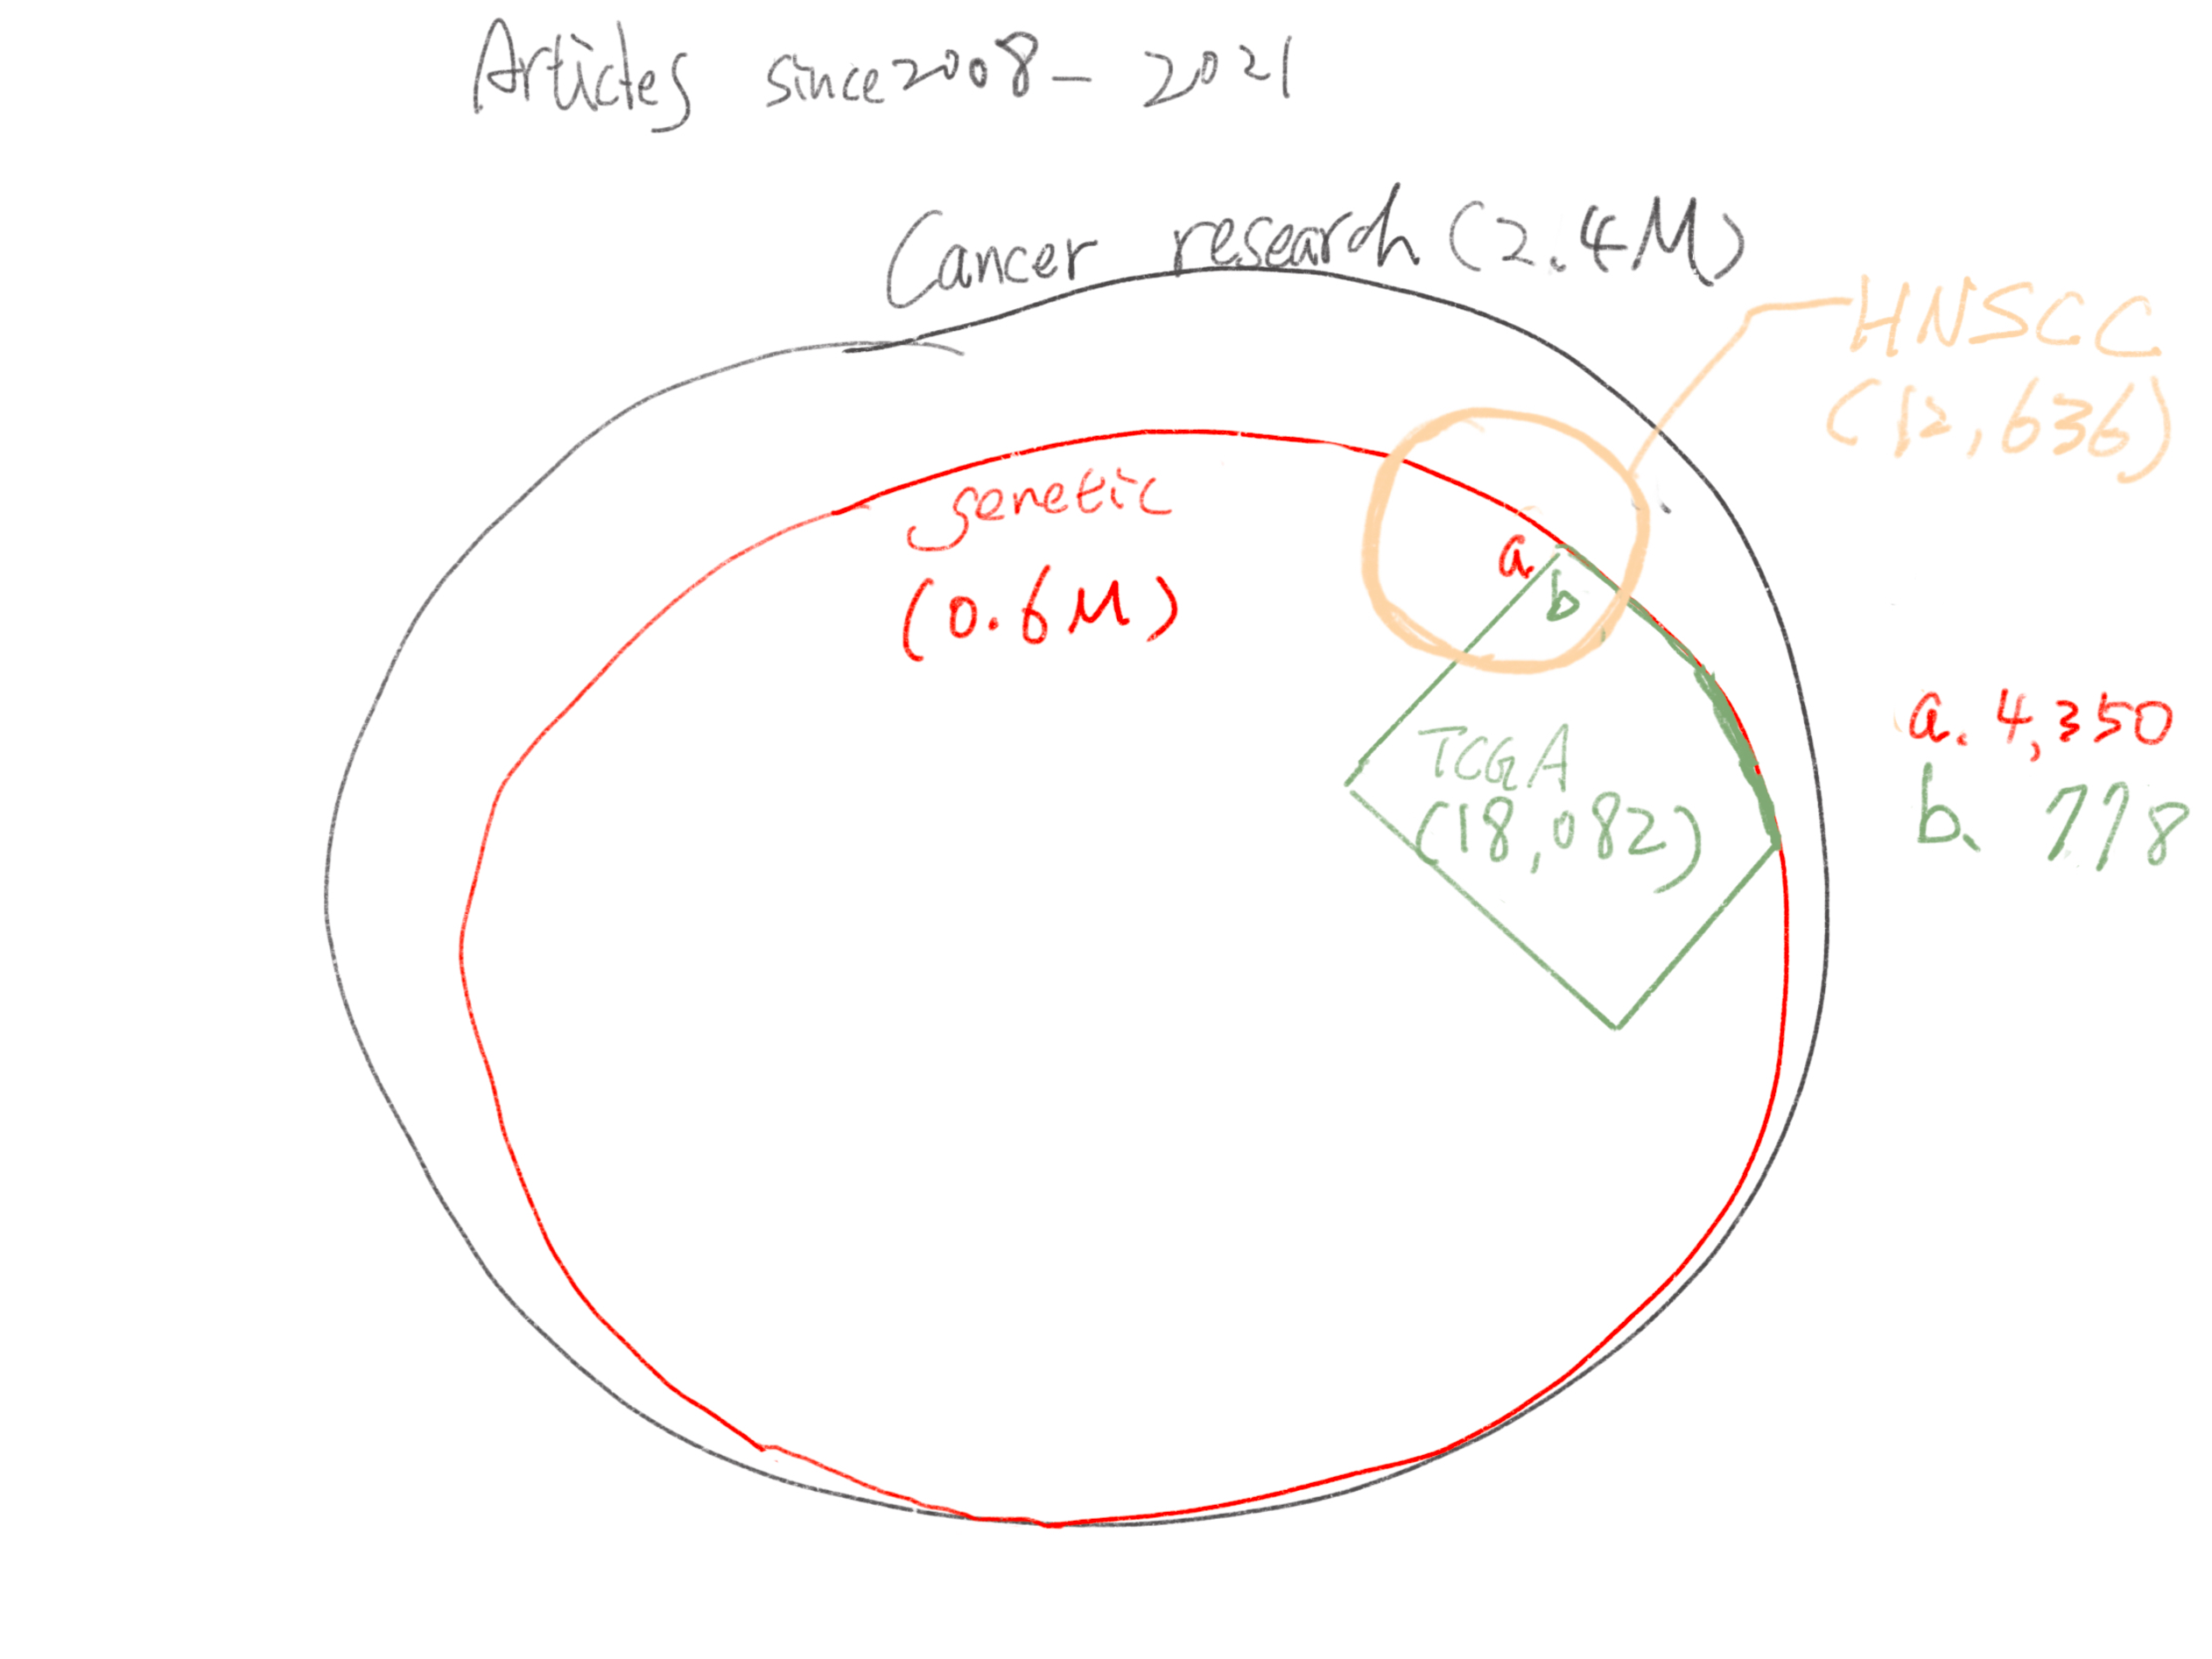
\includegraphics[width=14cm]{Answer_2-1.pdf}
%\label{figure:fig_embase}
\end{figure}
\clearpage
%778/4350 = 17.9\% using TCGA data
%There is 374 genes in the oral cancer gene database of Indian HNSCC; http://www.bioinformation.net/006/97320630006169.pdf
%http://www.actrec.gov.in/OCDB/index.htm

Despite of other databases carrying HNSCC genomics and clinical data we found, such as MSKCC (151 cases), Broad (74 cases), Johns Hopkins (32 cases), MD Anderson (40 cases), and NCBI GEO datasets (e.x. GSE2837, 40 cases; GSE6631, 22 cases; GSE31056, 23 cases)\cite{Cerami2012b}\cite{Gao2013a}. However,  MSKCC, Broad and Johns Hopkins databases were processed the whole-exome sequencing instead of whole-genome sequencing in TCGA database.

There is several useful web-tools for survival analysis, such as cBioportal\cite{Cerami2012b}\cite{Gao2013a}, KM-Plotter\cite{Gyorffy2010}, and SurvExpress\cite{Aguirre-Gamboa2013}. According to the citing articles\cite{Wu2020} and their online documents, the back-end database was collected from TCGA, the European Genome-phenome Archive (EGA)\cite{Lappalainen2015} and NCBI GEO (available at https://www.ncbi.nlm.nih.gov/gds) datasets. Furthermore, almost all of their survival data came from TCGA database.
%GEO (few survival features, less than 100 participate in each GSE dataset)
%GSE31056, GSE2837 (Prognoscan)
%there is survival feature: A total of 44 patients (22 HNSCC samples and 22 normal samples) were obtained from GSE6631
%有文章為證1. Lawrence, M. S. et al. Comprehensive genomic characterization of head and neck squamous cell carcinomas. Nature 517, 576–582 (2015).\cite{Lawrence2015a}
%datasets for each cancer type that include exactly the same prediction and outcome variables and consider comparable target populations. Currently, such data is simply not available.

Conclusion: TCGA database is representative for HNSCC.

\end{MyColorPar}

\subsection*{2-2}
Can be the found positive and negative prognostic genes underlined by comparable studies using other databases than TCGA?

\begin{MyColorPar}{blue}
Answer

We appreciate the reviewer for the critical comments and thank for your agreement of our experiments in the validation phase.....
GSE2837 (GEO) from PrognoScan: http://dna00.bio.kyutech.ac.jp/PrognoScan-cgi/PrognoScan.cgi \cite{Mizuno2009a}
https://www.ncbi.nlm.nih.gov/geo/query/acc.cgi?acc=GSE2837 \cite{Chung2006}
DKK1, CAMK2N1, STC2, PGK1, SURF4, USP10, NDFIP1, FOXA2, STIP1, DKC1;
ZNF557, ZNF266, IL19, MYO1H, FCGBP, LOC148709, EVPLL, PNMA5, IQCN, KIAA1683, NPB
Relapse Free Survival (RFS) in GSE2837 (not available on the TCGA dataset)
microarray gene expression experiments (Affymetrix X3P chips U133\_X3P)
cohort: VUMC, VAMC, UTMDACC (1992-2005), published on 2006
40 HNSCC samples
cohort n=28 in the following probes of genes with survival significance:
17 out of 20 candidates => 10 genes achieve similar positive and negative prognostic effect comparable with our candidate genes, however, its group separation was be cut by a skewed manner
FCGBP (P-value 0.005658 of KM plot)
FOXA2 (0.001587)


\end{MyColorPar}

\subsection*{2-3}
Could the authors summarize the elements of the workflow that could be used on any database independently from TCGA?


\begin{MyColorPar}{blue}
Answer

We appreciate the reviewer for the critical comments and thank for your agreement of our experiments in the validation phase.....
Currently, less HNSCC dataset is available worldwide (Indian?) => GEO
generalized use is fine for this workflow, it needs to modify the R code to adapt 
%能否套用在別的 database,可以,但需要 d/l raw microarray or RNA-seq 而且需要標準化(fpkm or RSEM)
It made the messenger \acrshort{rnaseq} matrix with log2 transformed for the downstream analysis, as described in their reference\cite{RSEM2016}.?)
Moreover, we are planning to expand this workflow for pan-cancer studies (other cancer types in the TCGA database).
the elements of the workflow: ...
\end{MyColorPar}


\subsection*{2-4}
Please shortly explain the TCGA database in the Introduction and summarize the advantages of its use.

\begin{MyColorPar}{blue}
Answer

We appreciate the reviewer for the critical comments and thank for your agreement of our experiments in the validation phase.....
*** We modified the introduction according to reviewer's comment...
https://www.cancer.gov/about-nci/organization/ccg/research/structural-genomics/tcga/publications
The Cancer Genome Atlas (TCGA): The TCGA consortium, which is a National Institute of Health (NIH) initiative, makes publicly available molecular and clinical information for more than 30 types of human cancers including exome (variant analysis), single nucleotide polymorphism (SNP), DNA methylation, transcriptome (mRNA), microRNA (miRNA) and proteome. Sample types available at TCGA are: primary solid tumors, recurrent solid tumors, blood derived normal and tumor, metastatic, and solid tissue normal.


\end{MyColorPar}



\subsection*{3-1}
Comments from the reviewer \#3

Must be improved:
Is the research design appropriate?
Are the results clearly presented?
Are the conclusions supported by the results?

3-1) Only computer computing in this research to support 20 candidate biomarkers, DKK1, CAMK2N1, STC2, PGK1, SURF4, USP10, NDFIP1, FOXA2, STIP1, DKC1, as well as ZNF557, ZNF266, IL19, MYO1H, FCGBP, LOC148709, EVPLL, PNMA5, IQCN (previous name as KIAA1683), and NPB, are all heavily associated with the prognosis of OS.

There is little information provided. The authors should provide more evidence to support this article.
%  Once the authors identify TMSB4X as a target, the rest of the analysis seems fine, but their rationale for looking into TMSB4X is not strongly supported by the available data.

\begin{MyColorPar}{blue}
Answer

We appreciate the reviewer for the critical comments and thank for your agreement of our experiments in the validation phase.....

DKK1 has the P-value 1.99328e-07 of multivariable Cox proportional hazards regression model, which was reported by network-based biomarkers research tools (SurvNet, accessed at http://bioinformatics.mdanderson.org/main/SurvNet; saved as supplementary file SurvNet_HNSCC_result.tsv)\cite{Li2012a}. %gene regulatory or protein interaction network
% cited by 10 articles
% he P-values pi from a univariable Cox proportional hazards regression model, which quantifies how significantly the molecular profiling data of the gene correlate with the patient survival data. 
% SurvNet also calculates the mutivariable Cox P-values for each subnetwork (a group of genes) to validate their clinical utility.
The network files are in a '.dot' format that can be visualized by GraphViz (http://www.graphviz.org)

a) Embase searching; %https://www.ncbi.nlm.nih.gov/research/pubtator/?view=docsum&query=CAMK2N1%20head%20and%20neck%20cancer
\cite{Wei2019}
through the PubMed searching, the remark on table 1 and table 2 presents the cancer research articles related to our candidate genes.

% bad guy
until 2020 1. Wei, R. et al. Analyzing the prognostic value of DKK1 expression in human cancers based on bioinformatics. Ann. Transl. Med. 8, 552 (2020).
\cite{Tang2019}\cite{Wei2020a}
https://www.cancer.gov/about-nci/organization/ccg/research/structural-genomics/tcga/publications
http://gepia2.cancer-pku.cn/detail.php?gene=DKK1
DKK1: 13 results of HNSCC \cite{Shi2014}\cite{Gao2018}\cite{Chakraborty2020}\cite{Hu2020}\cite{Wei2020}
CAMK2N1: 26 results of cancer: ; 1 HNSCC cell line (CAL-27)\cite{Li2018b}
STC2: \cite{Ma2020}
PGK1: glycolysis enzyme is responsive in cisplatin-resistant oral squamous cell carcinoma cell line\cite{Nakamura2005}
SURF4: patients with tumors (not HNSCC) exhibiting high SURF4 expression had significantly shorter overall survival than low SURF4 expression.\cite{Kim2018a}
USP10: one of autophagy related genes for HNSCC prognosis prediction.\cite{Ren2020}
% 13 ARGs (GABARAPL1, ITGA3, USP10, ST13, MAPK9, PRKN, FADD, IKBKB, ITPR1, TP73, MAP2K7, CDKN2A, and EEF2K) with prognostic value were identified in HNSCC patients
NDFIP1, was reported as candidate biomarker for hepatocellular carcinoma\cite{Zhang2019a} and breast cancer\cite{Tian2020}.
%  the adaptor protein Nedd4-family interacting protein 1 (NDFIP1) plays a key role in the ubiquitination and nuclear translocation of PTEN. It represses cell proliferation of melanoma and thus acts as a tumor suppressor.(PMID: 29333944)
FOXA2: hihger expression is significantly associated with the poor prognosis of HNSCC\cite{Shen2017a}.
%  + 0.0256 × cg03774514 FOXA2 => "+" coefficients; higher prognostic score was significantly associated with shorter survival in the training set; 
STIP1, increased expression of STIP1, detectable auto-antibody in serum sample, may indicate poor survival outcome in ovarian cancer patients\cite{Chao2013}\cite{Cho2014}. The auto-antibody against STIP1 could be a useful biomarker for esophageal squamous cell carcinoma\cite{Xu2017}.
DKC1, DKC1 (dyskeratin) is related with HNSCC\cite{Smith2010}.
%is the tumor suppressor gene in HNSCC

% good guy
ZNF557, oncogenic human herpesviruses, EBV and KSHV are silenced by SZF1 and ZNF557, two members of the KRAB-ZFP repressor family\cite{Li2018c}.
ZNF266, % or ZNF16, HZF1?
those genes were reported at following, 
IL19 in esophageal squamous cell carcinoma\cite{Hsing2013},
MYO1H associated mandibular prognathism\cite{Sun2018}, 
FCGBP in thyroid cancer\cite{Griffith2006}, 
?LOC148709?, 
EVPLL in cDNA project,
PNMA5 promotes apoptosis signaling in HeLa and MCF-7 cells\cite{Lee2016}, 
IQCN (previous name as KIAA1683), and 
NPB (Neuropeptide B) is endogenous ligand of the G protein-coupled receptors, named GPR7\cite{Andreis2005}, which is associated with prostate cancer prognosis\cite{Cottrell2007}. 



b) (ok) SurvExpress
%試試利用手動找到類似的結果 
Web resource for Biomarker comparison and validation of Survival gene expression data. 
Dataset: HNSC - TCGA Head and Neck squamous cell carcinoma June 2016 (dup=all, data=raw),(only TCGA June 2016, n=502) \cite{Aguirre-Gamboa2013}
%有類似的結果:
DKK1, CAMK2N1, STC2, PGK1, SURF4, USP10, NDFIP1, STIP1, DKC1,ZNF557, ZNF266, FCGBP;
%沒有
FOXA2, IL19, MYO1H, LOC148709, EVPLL, PNMA5, IQCN, KIAA1683, NPB
it supposed that ...
%因為 cutoff 不適當,這也就是我們 p-value Tex 的設計目的與強項
 (TCGA)(***please see Figure \label{fig_SurvExpress})

%x c) CCLE_RNAseq_rsem_genes_tpm_20180929.txt.gz
We provide more evidences mentioned above to support the prognostic impact of these candidate genes. It needs to be further validated.
\end{MyColorPar}

% the end of response letter

\section{Highlights}
Highlights
\begin{itemize}
    \item The R script program could automatically scan protein-coding genes and generate the Kaplan-Meier plots and Cox's univariate/multivariate tables.
    \item Using a serial cut from 30\% to 70\% percentile of the cohort, it could find the least P-value cutoff of the Kaplan-Meier analysis for each gene expression.
    \item Our analysis could discover the pronounced biomarkers, which impact HNSCC's survival under the stringent Bonferroni adjustment.
\end{itemize}

%\reftitle{References}

% Please provide either the correct journal abbreviation (e.g. according to the “List of Title Word Abbreviations” http://www.issn.org/services/online-services/access-to-the-ltwa/) or the full name of the journal.
% Citations and References in Supplementary files are permitted provided that they also appear in the reference list here. 

%\externalbibliography{yes}
%\bibliography{your_external_BibTeX_file}
\bibliographystyle{unsrt} %model1-num-names}
\bibliography{TCGA_margin_cutoff.bib}

\end{document}

